\documentclass{article}
\usepackage[utf8]{inputenc}
\usepackage{xcolor}
\usepackage{colortbl}
\usepackage{graphicx}
\usepackage{tikz}
\usepackage{lmodern}
\usepackage{amssymb,amsmath}
\usepackage{ifxetex,ifluatex}
\usepackage{fixltx2e} % provides \textsubscript
\usepackage{ngerman}
\usepackage{float}
\usepackage{caption}
\usepackage{subcaption}


\PassOptionsToPackage{hyphens}{url} % url is loaded by hyperref
\usepackage[unicode=true]{hyperref}

\usepackage{color}
\usepackage{fancyvrb}

\usepackage{mathtools}

\usepackage[a4paper, margin=3cm]{geometry}

\DeclarePairedDelimiter\floor{\lfloor}{\rfloor}
\newcommand*{\qed}{\hfill\ensuremath{\blacksquare}\\}%

% set default figure placement to htbp
\makeatletter

\title{FOP Projekt Wintersemester 2019/20}
\author{Yannik Sebastian Hayn, Julian Imhof,\\ Erik Prescher, Lennart Schmidt}
\makeatletter
\renewcommand*{\ps@plain}{%
  \let\@mkboth\@gobbletwo
  \let\@oddhead\@empty
  \def\@oddfoot{%
    \reset@font
    \hfil
    \thepage
    % \hfil % removed for aligning to the right
  }%
  \let\@evenhead\@empty
  \let\@evenfoot\@oddfoot
}
\usepackage{listings}
\lstset{language=Java,
  showspaces=false,
  showtabs=false,
  breaklines=true,
  showstringspaces=false,
  breakatwhitespace=true,
  basicstyle=\ttfamily
}
\makeatother
\pagestyle{plain}

\begin{document}
\maketitle
\section{Aufgabe 6.1.5 Theorie}
\subsection{Azyklischer Graph}
Da nur ein gerichteter Graph azyklisch sein kann, der hier gegebene Graph allerdings nicht gerichtet ist, kann er folglich auch nicht azyklisch sein.\\
 Im Folgenden gehen wir allerdings davon aus, dass auch ein nicht gerichteter Graph azyklisch sein k\"onne. Dabei nehmen wir an, dass ein Zyklus aus mindestens drei Nodes bestehen muss und der Zyklus \"uber $n - 1$ Kanten durchlaufen werden k\"onnen muss, ohne dabei zwei mal \"uber eine Kante zu gehen, wobei $n = Anzahl der Nodes$ ist.\\
Im Folgenden zeigen wir, dass der Graph zyklisch sein kann.\\

Betrachten wir einmal die einfachste Idee, um einen Zyklus zu erzeugen: Ein Kreisverkehr aus mehreren Stra{\ss}enkarten.
\begin{figure}[H]
	\centering
	\begin{subfigure}{.5\textwidth}
		\centering
		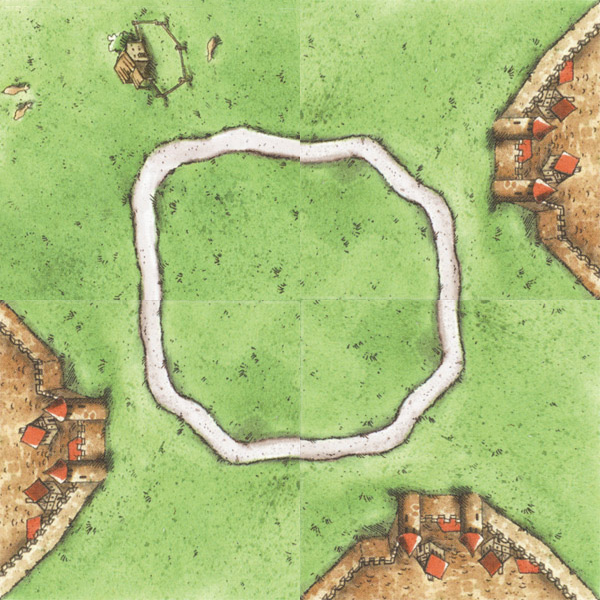
\includegraphics[width=0.9\textwidth]{Zyklischer_Graph.png}
		\caption{v.l.n.r. Pl\"attchen: V, J, J, J}
	\end{subfigure}%
	\begin{subfigure}{.5\textwidth}
		\centering
		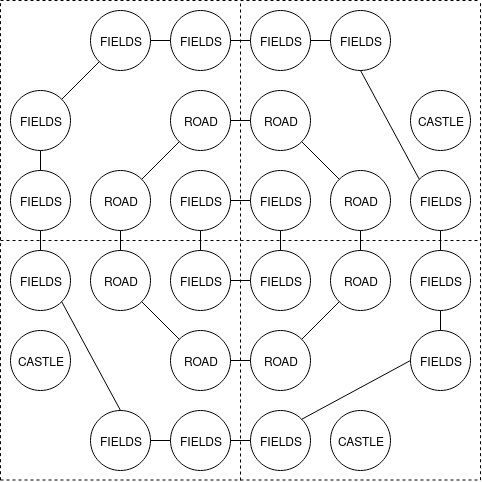
\includegraphics[width=0.9\textwidth]{Zyklischer_Graph1.png}
		\caption{zugeh\"origer Graph}
	\end{subfigure}
	\caption{Eine einfache M\"oglichkeit mit wenigen Pl\"attchen viele Zyklen zu erzeugen}
\end{figure}
Wie man direkt sehen kann, sind nur durch diese 4 Karten bereits 3 Zyklen entstanden.\qed

Wenn man diese Idee ein bisschen weiter f\"uhrt, kommt man relativ schnell zu dem Schluss, dass der Graph in den allermeisten F\"allen sp\"atestens bei Spielende zyklisch sein wird.

\section{Zusammenhangskomponenten}
F\"ur jedes Pl\"attchen $p$ gilt, dass es theoretisch maximal 9 Teilmengen von verschiedenen Zusammenhangskomponenten haben kann.
\begin{figure}[H]
	\centering
	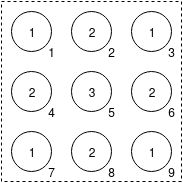
\includegraphics[width=0.3\textwidth]{aufgabe2_0.png}
	\caption{zeigt alle maximal m\"oglichen Zusammenhangskomponenten eines einzelnen Pl\"attchens}
\end{figure}
F\"ur $k$ nicht verbundene Pl\"attchen gilt also:
\begin{align*}
n &\leq 9 * k\\
\end{align*}
Nur die Knoten eines neu angelegten Pl\"attchens k\"onnen eine neue Zusammenhangskomponente bilden, wenn sie nicht Teil einer Kante mit einem bereits gelegten Pl\"attchen sind. Da ein neues Pl\"attchen aber nur an mindestens einem alten Pl\"attchen angelegt werden kann, gilt, dass mindestens drei Knoten an einer gemeinsamen Kante liegen, und somit maximal 6 neue Zusammenhangskomponenten existieren k\"onnen. 
\begin{figure}[H]
	\centering
	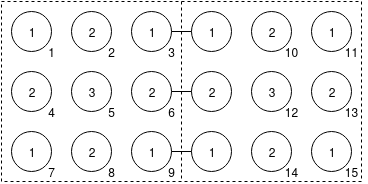
\includegraphics[width=0.5\textwidth]{aufgabe2_1.png}
	\caption{zeigt, dass nur maximal 6 neue Zusammenhangskomponenten geben kann}
\end{figure}
Somit gilt, wenn man ein neues Pl\"attchen an nur einem alten anlegt:
\begin{align*}
n &\leq 9 + 6*(k-1)
\end{align*}
Legt man ein neues Pl\"attchen hingegen an 2 oder mehr Pl\"attchen an, so ergeben sich immer weniger als $6$ potentielle neue Zusammenhangskomponenten, wie man Abbildung 4 entnehmen kann.
\begin{figure}[H]
	\centering
	\begin{subfigure}{.5\textwidth}
		\centering
		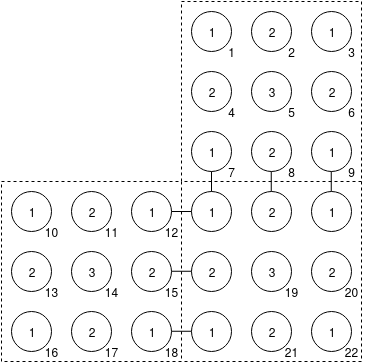
\includegraphics[width=0.9\textwidth]{aufgabe2_2.png}
	\end{subfigure}%
	\begin{subfigure}{.5\textwidth}
		\centering
		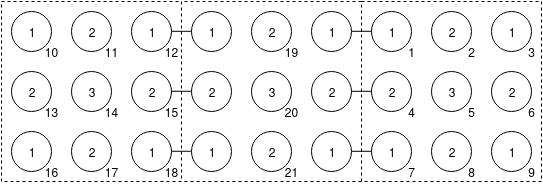
\includegraphics[width=0.9\textwidth]{aufgabe2_3.png}
	\end{subfigure}\\
	\begin{subfigure}{.5\textwidth}
		\centering
		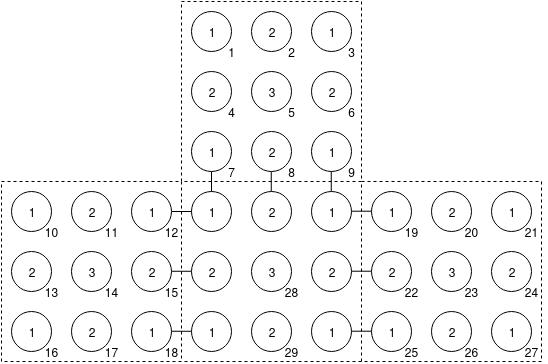
\includegraphics[width=0.9\textwidth]{aufgabe2_4.png}
	\end{subfigure}%
	\begin{subfigure}{.5\textwidth}
		\centering
		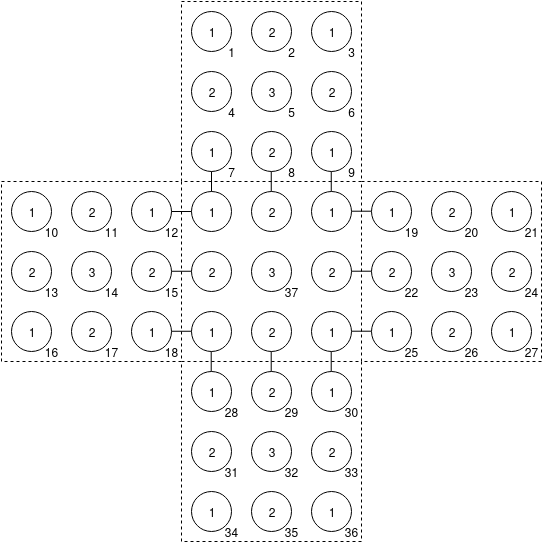
\includegraphics[width=0.9\textwidth]{aufgabe2_5.png}
	\end{subfigure}
	\caption{Alle M\"oglichkeiten ein neues Pl\"attchen an mehr als 2 bereits gelegte Pl\"attchen anzulegen}
\end{figure}
Somit gilt die oben ermittelte Ungleichung also f\"ur alle an das Startpl\"attchen angelegte Pl\"attchen.
\begin{align*}
n &\leq 9 + 6*(k-1)\\
\Leftrightarrow n &\leq 9 + 9*(k-1)\\
\Leftrightarrow n &\leq 9*(k-1+1)\\ 
\Leftrightarrow n &\leq 9k\\
\end{align*}
Somit zeigt sich, dass die gegenene Ungleichnug nicht die Pr\"aziseste, allerdings korrekt ist.
\qed

\end{document}
